\documentclass[12pt]{article}

\usepackage{ishn}

\makeindex[intoc]

\begin{document}

\hypersetup{pageanchor=false}
\begin{titlepage}
	\begin{center}
		\vspace*{1em}
		\Huge
		\textbf{III Combinatorics}

		\vspace{1em}
		\large
		Ishan Nath, Michaelmas 2024

		\vspace{1.5em}

		\Large

		Based on Lectures by Prof. Imre Leader

		\vspace{1em}

		\large
		\today
	\end{center}
	
\end{titlepage}
\hypersetup{pageanchor=true}

\tableofcontents

\newpage

%lecture 1

\setcounter{section}{-1}

\section{Introduction}%
\label{sec:intro}

We have the following list of things.
\begin{enumerate}[1:]
	\item Set systems.
	\item Isoperimetric inequalities.
	\item Intersection families.
\end{enumerate}

Books include `Combinatorics' by Bollob\'as, and `Combinatorics of Finite Sets', by Anderson.

\newpage

\section{Set Systems}%
\label{sec:ss}

Let $X$ be a set. A \emph{set system}\index{set system} on $X$, also called a family of subsets of $X$, is a family $\mathcal{A} \subseteq \mathcal{P}(X)$. For example,
\[
	X^{(r)} = \{A \subseteq X \mid |A| = r \}.
\]
Usually, $X = [n] = \{1, 2, \ldots, n\}$, so $|X^{(r)}| = \binom nr$. Thus,
\[
	[4]^{(2)} = \{12, 13, 14, 23, 24, 34\}.
\]

We make $\mathcal{P}(X)$ into a graph by joining $A$ and $B$ if $|A \triangle B| = 1$. This is the \emph{discrete cube}\index{discrete cube} $Q_n$.

Literally just a cube.

\[
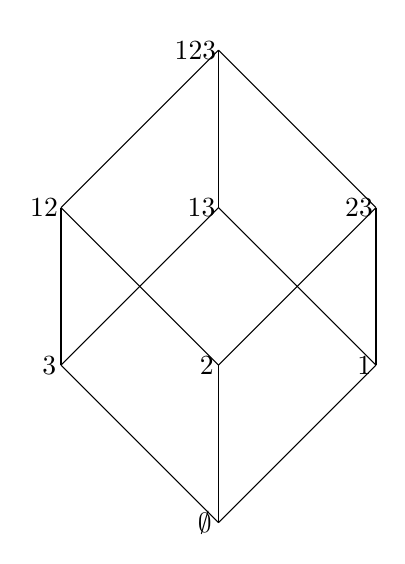
\begin{tikzpicture}[scale=2, every node/.style={circle, draw, fill=black, inner sep=0pt, minimum width=4pt}]

% Define the coordinates for the vertices of the cube
\coordinate (000) at (0,0);
\coordinate (001) at (1,1);
\coordinate (011) at (1,2);
\coordinate (010) at (0,1);
\coordinate (100) at (-1,1);
\coordinate (101) at (0,2);
\coordinate (111) at (0,3);
\coordinate (110) at (-1,2);

% Draw edges of the cube
\draw (000) -- (001);
\draw (001) -- (011);
\draw (011) -- (010);
\draw (010) -- (000);

\draw (100) -- (101);
\draw (101) -- (111);
\draw (111) -- (110);
\draw (110) -- (100);

\draw (000) -- (100);
\draw (001) -- (101);
\draw (011) -- (111);
\draw (010) -- (110);

% Place the vertices as small black circles

\node[draw=none, fill=none, anchor=east] at (000) {$\emptyset$};
\node[draw=none, fill=none, anchor=east] at (001) {1};
\node[draw=none, fill=none, anchor=east] at (011) {23};
\node[draw=none, fill=none, anchor=east] at (010) {2};
\node[draw=none, fill=none, anchor=east] at (100) {3};
\node[draw=none, fill=none, anchor=east] at (101) {13};
\node[draw=none, fill=none, anchor=east] at (111) {123};
\node[draw=none, fill=none, anchor=east] at (110) {12};

\end{tikzpicture}
\]
Alternatively, can view $Q_n$ as an $n$-dimensional unit cube $\{0, 1\}^n$, by identifying e.g. $\{1, 3\}$ with the binary string $101000\cdots$.
\[
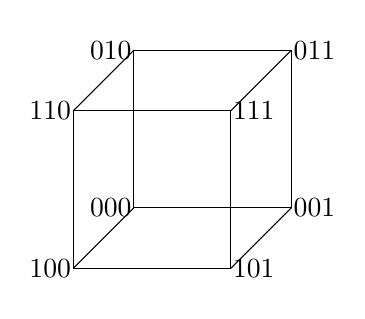
\begin{tikzpicture}[scale=2, every node/.style={circle, draw, fill=black, inner sep=0pt, minimum width=4pt}]

% Define the coordinates for the vertices of the cube
\coordinate (000) at (0,0,0);
\coordinate (001) at (1,0,0);
\coordinate (011) at (1,1,0);
\coordinate (010) at (0,1,0);
\coordinate (100) at (0,0,1);
\coordinate (101) at (1,0,1);
\coordinate (111) at (1,1,1);
\coordinate (110) at (0,1,1);

% Draw edges of the cube
\draw (000) -- (001);
\draw (001) -- (011);
\draw (011) -- (010);
\draw (010) -- (000);

\draw (100) -- (101);
\draw (101) -- (111);
\draw (111) -- (110);
\draw (110) -- (100);

\draw (000) -- (100);
\draw (001) -- (101);
\draw (011) -- (111);
\draw (010) -- (110);

% Place the vertices as small black circles

\node[draw=none, fill=none, anchor=east] at (000) {000};
\node[draw=none, fill=none, anchor=west] at (001) {001};
\node[draw=none, fill=none, anchor=west] at (011) {011};
\node[draw=none, fill=none, anchor=east] at (010) {010};
\node[draw=none, fill=none, anchor=east] at (100) {100};
\node[draw=none, fill=none, anchor=west] at (101) {101};
\node[draw=none, fill=none, anchor=west] at (111) {111};
\node[draw=none, fill=none, anchor=east] at (110) {110};


\end{tikzpicture}
\]

Say $\mathcal{A} \subseteq \mathcal{P}(X)$ is a \emph{chain}\index{chain} if, for all $A, B \in \mathcal{A}$, $A \subseteq B$ or $B \subseteq A$. For example,
\[
	\mathcal{A} = \{23, 12357, 1235, 123567\}
\]
is a chain.

Say $\mathcal{A}$ is an \emph{antichain}\index{antichain} if, for all $A, B \in \mathcal{A}$ and $A \neq B$, we have $A \not \subseteq B$. For example, $\mathcal{A} = \{23, 137\}$ is an antichain.

How large can a chain be? We can achieve $|\mathcal{A}| = n+1$ by taking
\[
	\mathcal{A} = \{ \emptyset, 1, 12, 123, \ldots, [n]\}
\]
Cannot beat this as each $0 \leq r \leq n$, $\mathcal{A}$ can contain at most one $r$-set (a member of $X^{(r)}$).

How large can an antichain be? We can achieve $|\mathcal{A}| = n$, e.g. $\mathcal{A} = \{1, 2, \ldots, n\}$. More generally, we can take $\mathcal{A} = X^{(r)}$, and the best is when $r = \lfloor n/2 \rfloor$.

% lecture 2

\begin{theorem}[Sperner's Lemma]
	Let $\mathcal{A} \subseteq \mathcal{P}(X)$ be an antichain. Then,
	\[
		|\mathcal{A}| \leq \binom{n}{\lfloor n/2 \rfloor}.
	\]
\end{theorem}

The idea is follows: we know that a chain meets a layer in at most one point, since a layer is an antichain. If we decompose the cube into chains, we have at most one element of an antichain in each chain.

\begin{proofbox}
	We will decompose $\mathcal{P}(X)$ into $\binom n {\lfloor n/2 \rfloor}$ chains, then we are done. To achieve this, it is sufficient to find:
	\begin{enumerate}[(i)]
		\item For each $r < n/2$, a matching from $X^{(r)}$ to $X^{(r + 1)}$.
		\item For each $r \geq n/2$, a matching from $X^{(r)}$ to $X^{(r - 1)}$.
	\end{enumerate}
	Then we put these together to form our chains; each passing through $X^{(\lfloor n/2 \rfloor)}$.

	By taking complements, it is enough to prove (i).

	Let $G$ be the bipartite subgraph of $Q_n$ spanned by $X^{(r)} \cup X^{(r + 1)}$: we seek a matching from $X^{(r)}$ to $X^{(r + 1)}$.

	For any $S \subseteq X^{(r)}$, the number of edges from $S$ to $\Gamma(S)$ is $|S|(n - r)$, since each edge in $S$ has $n - r$ edges.

	Moreover there are at most $|\Gamma(S)|(r + 1)$ edges, counting from $\Gamma(S)$. Therefore,
	\[
	|\Gamma(S)| \geq \frac{|S|(n-r)}{r + 1} \geq |S|.
	\]
	So we are done, by Hall's matching theorem.
\end{proofbox}

\begin{center}
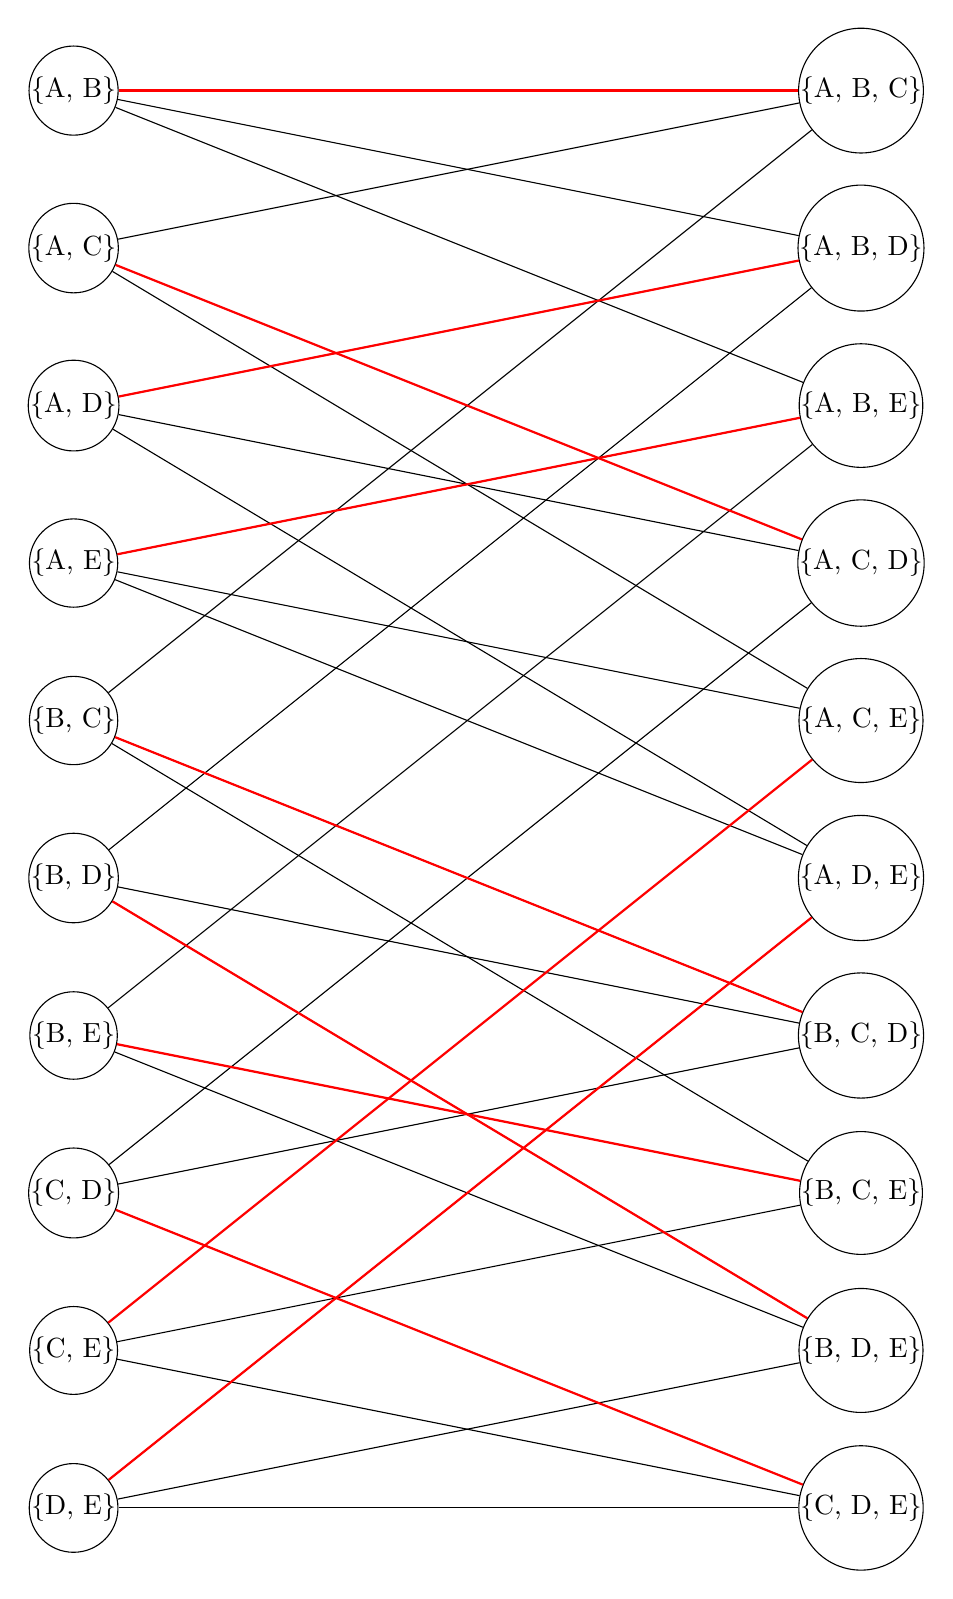
\begin{tikzpicture}[scale=1,>=latex, every node/.style={circle, draw, minimum size=1mm, inner sep=0pt}]

    % Define the 2-element subsets X^{(2)} (left side)
    \node (AB) at (-5, 9) {\{A, B\}};
    \node (AC) at (-5, 7) {\{A, C\}};
    \node (AD) at (-5, 5) {\{A, D\}};
    \node (AE) at (-5, 3) {\{A, E\}};
    \node (BC) at (-5, 1) {\{B, C\}};
    \node (BD) at (-5, -1) {\{B, D\}};
    \node (BE) at (-5, -3) {\{B, E\}};
    \node (CD) at (-5, -5) {\{C, D\}};
    \node (CE) at (-5, -7) {\{C, E\}};
    \node (DE) at (-5, -9) {\{D, E\}};

    % Define the 3-element subsets X^{(3)} (right side)
    \node (ABC) at (5, 9) {\{A, B, C\}};
    \node (ABD) at (5, 7) {\{A, B, D\}};
    \node (ABE) at (5, 5) {\{A, B, E\}};
    \node (ACD) at (5, 3) {\{A, C, D\}};
    \node (ACE) at (5, 1) {\{A, C, E\}};
    \node (ADE) at (5, -1) {\{A, D, E\}};
    \node (BCD) at (5, -3) {\{B, C, D\}};
    \node (BCE) at (5, -5) {\{B, C, E\}};
    \node (BDE) at (5, -7) {\{B, D, E\}};
    \node (CDE) at (5, -9) {\{C, D, E\}};

    % Draw edges representing the bipartite connections (subset relationships)
    \draw (AB) -- (ABC);
    \draw (AB) -- (ABD);
    \draw (AB) -- (ABE);

    \draw (AC) -- (ABC);
    \draw (AC) -- (ACD);
    \draw (AC) -- (ACE);

    \draw (AD) -- (ABD);
    \draw (AD) -- (ACD);
    \draw (AD) -- (ADE);

    \draw (AE) -- (ABE);
    \draw (AE) -- (ACE);
    \draw (AE) -- (ADE);

    \draw (BC) -- (ABC);
    \draw (BC) -- (BCD);
    \draw (BC) -- (BCE);

    \draw (BD) -- (ABD);
    \draw (BD) -- (BCD);
    \draw (BD) -- (BDE);
    \draw (BE) -- (ABE);
    \draw (BE) -- (BCE);
    \draw (BE) -- (BDE);
    \draw (CD) -- (ACD);
    \draw (CD) -- (BCD);
    \draw (CD) -- (CDE);
    \draw (CE) -- (ACE);
    \draw (CE) -- (BCE);
    \draw (CE) -- (CDE);
    \draw (DE) -- (ADE);
    \draw (DE) -- (BDE);
    \draw (DE) -- (CDE);

    % Draw the matching edges
    \draw[red,thick] (AB) -- (ABC);
    \draw[red,thick] (AC) -- (ACD);
    \draw[red,thick] (AD) -- (ABD);
    \draw[red,thick] (AE) -- (ABE);
    \draw[red,thick] (BC) -- (BCD);
    \draw[red,thick] (BD) -- (BDE);
    \draw[red,thick] (BE) -- (BCE);
    \draw[red,thick] (CD) -- (CDE);
    \draw[red,thick] (CE) -- (ACE);
    \draw[red,thick] (DE) -- (ADE);

\end{tikzpicture}
\end{center}

When do we have equality in Sperner's? The above proof tells us nothing.

Our aim is to prove the following: if $\mathcal{A}$ is an antichain, then
\[
\sum_{r = 0}^n \frac{|\mathcal{A} \cap X^{(r)}|}{\binom nr} \leq 1.
\]
In other words, the percentages of each layer occupied add up to at most 1. This trivially implies Sperner's.

\subsection{Shadows}%
\label{sub:shadow}

For $\mathcal{A} \subseteq X^{(r)}$, the \emph{shadow}\index{shadow} of $\mathcal{A}$ is $\partial \mathcal{A} = \partial^- \mathcal{A} \subseteq X^{(r - 1)}$ defined by
\[
	\partial \mathcal{A} = \{ B \in X^{(r-1)} \mid B \subseteq A \text{ for some } A \in \mathcal{A}\}.
\]
For example, if $\mathcal{A} = \{123, 124, 134, 137\}$, then
\[
	\partial \mathcal{A} = \{12, 13, 23, 14, 24, 34, 17, 37\}.
\]

\begin{proposition}[Local LYM]
	Let $\mathcal{A} \subseteq X^{(r)}$. Then,
	\[
		\frac{|\partial \mathcal{A}|}{\binom{n}{r-1}} \geq \frac{|\mathcal{A}|}{\binom{n}{r}}.
	\]
\end{proposition}

So, the fraction of the local occupancy by $\partial \mathcal{A}$, is at least the occupancy by $\mathcal{A}$.

\begin{remark}
	LYM = Lubell, Meshalkin, Yamamoto.
\end{remark}

\begin{proofbox}
	We look at the number of $\mathcal{A}$ to $\partial \mathcal{A}$ edges in the bipartite graph $Q_n$; counting from above, there are exactly $|\mathcal{A}| r$.

	However counting from below, it is at most $|\partial \mathcal{A}|(n - r + 1)$. So,
	\[
		\frac{|\partial \mathcal{A}|}{|\mathcal{A}|} \geq \frac{r}{n - r + 1} = \frac{\binom n{r-1}}{\binom nr}.
	\]
	So we are done.
\end{proofbox}

\begin{remark}
	When do we have equality? We lose equality if an element in $\partial \mathcal{A}$ is connected to an element not in $\mathcal{A}$, so for this not to occur, we need that for all $A \in \mathcal{A}$, and $i \in A$, $j \not \in \mathcal{A}$, that $A - \{i\} \cup \{j\} \in \mathcal{A}$.

	But this is very strong, and in fact either $\mathcal{A} = \emptyset$ or $X^{(r)}$.
\end{remark}

\begin{theorem}[LYM Inequality]
	Let $A \subseteq \mathcal{P}(X)$ be an antichain. Then,
	\[
	\sum_{r = 0}^n \frac{|\mathcal{A} \cap X^{(r)}|}{\binom nr} \leq 1.
	\]
\end{theorem}

As a bit of notation, we write $\mathcal{A}_r$ for $\mathcal{A} \cap X^{(r)}$.

We will look at two proofs. The first idea is to bubble down with local LYM.

\begin{proofbox}
	Obviously
	\[
	\frac{|\mathcal{A}_n|}{\binom nn} \leq 1.
	\]
	Now, $\partial A_n$ and $\mathcal{A}_{n-1}$ are disjoint, as $\mathcal{A}$ is an antichain. So,
	\[
		\frac{|\partial \mathcal{A}_n|}{\binom n{n-1}} + \frac{|\mathcal{A}_{n-1}|}{\binom n{n-1}} = \frac{|\partial \mathcal{A}_n \cup \mathcal{A}_{n-1}|}{\binom n{n-1}} \leq 1,
	\]
	whence we get
	\[
		\frac{|\mathcal{A}_n|}{\binom nn} + \frac{|\mathcal{A}_{n-1}|}{\binom n{n-1}} \leq 1,
	\]
	by local LYM. We now continue again. Notice $\partial (\partial \mathcal{A}_n \cup \mathcal{A}_{n-1})$ is disjoint from $\mathcal{A}_{n-2}$, we find
	\[
		\frac{|\partial(\partial \mathcal{A}_n \cup \mathcal{A}_{n-1})|}{\binom n{n-2}} + \frac{|\mathcal{A}_{n-2}|}{\binom n{n-2}} \leq 1,
	\]
	whence
	\[
		\frac{|\partial \mathcal{A}_n \cup \mathcal{A}_{n-1}|}{\binom n{n-1}} + \frac{|\mathcal{A}_{n-2}|}{\binom n{n-2}} \leq 1.
	\]
	We can now continue inductively.
\end{proofbox}

When do we have equality? We must have had equality in each use of local LYM. Hence equality in LYM needs that the maximum $r$ with $\mathcal{A}_r \neq \emptyset$, then $\mathcal{A}_r = X^{(r)}$.

Hence equality in Sperner needs either $\mathcal{A} = X^{(n/2)}$, if $n$ is even, or $\mathcal{A} = X^{(\lfloor n/2 \rfloor)}$ or $X^{(\lceil n/2 \rceil)}$, for $n$ odd.

% lecture 3

Now time for another proof.

\begin{proofbox}
	Choose uniformly at random a maximal chain $\mathcal{C}$. For any $r$-set $A$, note that
	\[
	\mathbb{P}(A \in \mathcal{C}) = \frac{1}{\binom nr}.
	\]
	So for our antichain $\mathcal{A}$,
	\[
		\mathbb{P}(\mathcal{C} \text{ meets } \mathcal{A}_r) = \frac{|\mathcal{A}_r|}{\binom nr},
	\]
	as these events are disjoint. Hence, since $\mathcal{C}$ can meet $\mathcal{A}$ at one point at most,
	\[
		\mathbb{P}(\mathcal{C} \text{ meets } \mathcal{A}) = \sum_{r = 0}^n \frac{|\mathcal{A}_r|}{\binom nr},
	\]
	from which we get
	\[
	\sum_{r = 0}^n \frac{|\mathcal{A}_r|}{\binom nr} \leq 1.
	\]
\end{proofbox}

Equivalently, the number of maximal chains is $n!$, and the number through any fixed $r$-set is $r!(n-r)!$, so
\[
\sum_r |\mathcal{A}_r| r! (n-r)! \leq n!.
\]

We now return to shadows. For $\mathcal{A} \subseteq X^{(r)}$, we have
\[
|\partial \mathcal{A}| \geq |\mathcal{A}| \frac{r}{n - r + 1}.
\]
We know that equality is rare: it only happens for $\mathcal{A} = \emptyset$, or $X^{(r)}$. What happens in between?

In other words, given $|\mathcal{A}|$, how should we choose $\mathcal{A} \subseteq X^{(r)}$ to minimise $|\partial \mathcal{A}|$?

It is believable that if $|\mathcal{A}| = \binom kr$, then we should take $\mathcal{A} = [k]^{(r)}$. In between adjacent binomials, it is believable that we should take $[k]^{(r)}$, plus some $r$-sets in $[k+1]^{(r)}$.

\begin{exbox}
	For $\mathcal{A} \subseteq X^{(3)}$ with 
	\[
	|\mathcal{A}| = \binom 83 + \binom 42,
	\]
	we could take
	\[
		\mathcal{A} = [8]^3 \cup \{9 \cup B \mid B \in [4]^{(2)}\}.
	\]
\end{exbox}

In some ways our set $\mathcal{A}$ should be of minimal `order', under some ordering on $X^{(r)}$.

\subsection{Total Orders}%
\label{sub:to_xr}

Let $A, B$ be distinct $r$-sets, and say $A = a_1 \ldots a_r$, $B = b_1 \ldots b_r$, where $a_1 < \cdots < a_r$, $b_1 < \cdots < a_r$.

We say that $A < B$ in the \emph{lexographic}\index{lexographic ordering} or \emph{lex} ordering if for some $j$ we have $a_i = b_i$ for all $i < j$, and $a_j < b_j$. So lex cares about small elements.

\begin{exbox}
	Lex on $[4]^{(2)}$ orders the elements as $12, 13, 14, 23, 24, 34$.

	Lex on $[6]^{(3)}$ orders the elements as
	\begin{align*}
		123, &124, 125, 126, 134, 135, 136, 145, 146, 156, \\
		     &234, 235, 236, 245, 246, 256, 345, 346, 356, 456.
	\end{align*}
\end{exbox}

We say that $A < B$ in the \emph{colexographic}\index{colexographic ordering} or \emph{colex} ordering if for some $j$, we have $a_i = b_i$ for all $i > j$, and $a_j < b_j$. So colex cares about big elements.


\begin{exbox}
	Colex on $[4]^{(2)}$ orders the elements as $12, 13, 23, 14, 24, 34$.

	Colex on $[6]^{(3)}$ orders the elements as
	\begin{align*}
		123, &124, 134, 234, 125, 135, 235, 145, 245, 345, \\
		     &126, 136, 236, 146, 246, 346, 156, 256, 356, 456.
	\end{align*}
\end{exbox}

Note that in colex, $[n-1]^{(r)}$ is an initial segment of $[n]^{(r)}$. This is not true in lex.

This allows us to view colex as an enumeration of $\mathbb{N}^{(r)}$.

\begin{remark}
	$A < B$ in colex $\iff A^c < B^c$ in lex, with ground set ordering ordering reversed.
\end{remark}

Colex in particular may be the ordering we want to solve the above problem, minimizing $|\partial \mathcal{A}|$. Our aim will then be to show that initial segments of colex are the best for $\partial$, i.e. if $\mathcal{A} \subseteq X^{(r)}$ and $\mathcal{C} \subseteq X^{(r)}$ is the initial segment of colex with $|\mathcal{C}| = |\mathcal{A}|$, then
\[
|\partial \mathcal{C}| \leq |\partial \mathcal{A}|.
\]
In particular,
\[
	|\mathcal{A}| = \binom kr \implies |\partial \mathcal{A}| = \binom k{r-1}.
\]
\subsection{Compression}%
\label{sub:comp}

The idea is to try to transform $\mathcal{A} \subseteq X^{(r)}$ into some $\mathcal{A}\ \subseteq X^{(r)}$ such that:
\begin{enumerate}[(i)]
	\item $|\mathcal{A}'| = |\mathcal{A}|$.
	\item $|\partial \mathcal{A}'| \leq |\partial \mathcal{A}|$.
	\item $\mathcal{A}'$ looks more like $\mathcal{C}$ than $\mathcal{A}$ did.
\end{enumerate}

Ideally, we would like a family of such `compressions'
\[
\mathcal{A} \to \mathcal{A}' \to \cdots \to \mathcal{B},
\]
such that either $\mathcal{B} = \mathcal{C}$, or $\mathcal{B}$ is so similar to $\mathcal{C}$ that we can directly check that
\[
|\partial \mathcal{B}| \geq |\partial \mathcal{C}|.
\]

% lecture 4

The fact that colex prefers 1 to 2 inspires the following: fix $1 \leq i < j \leq n$. The \emph{$ij$-compression}\index{compression} $C_{ij}$ is defined as follows:

For $A \in X^{(r)}$, set
\[
C_{ij}(A) =
\begin{cases}
	A \cup i - j &\text{if $j \in A$, $i \not \in A$ },\\
	A &\text{else.}
\end{cases}
\]
For $\mathcal{A} \subseteq X^{(r)}$, set
\[
	C_{ij}(\mathcal{A}) = \{ C_{ij}(A) \mid A \in \mathcal{A}\} \cup \{A \in \mathcal{A} \mid C_{ij}(A) \in \mathcal{A}\}.
\]
%For example, ....
So $C_{ij}(\mathcal{A}) \subseteq X^{(r)}$, and $|C_{ij}(\mathcal{A})| = |\mathcal{A}|$. Say $\mathcal{A}$ is $ij$-compressed if $C_{ij}(\mathcal{A}) = \mathcal{A}$.

\begin{lemma}
	Let $\mathcal{A} \subseteq X^{(r)}$, and $1 \leq i < j \leq n$. Then
	\[
	|\partial C_{ij}(\mathcal{A})| \leq |\partial\mathcal{A}|.
	\]
\end{lemma}

\begin{proofbox}
	Write $\mathcal{A}'$ for $C_{ij}(\mathcal{A})$, and let $B \in \partial \mathcal{A}' - \partial \mathcal{A}$. We will show that $i \in B, j \not \in B$, and $B \cup j - i \in \partial \mathcal{A} - \partial \mathcal{A}'$, which will show that we are done.

	We have that $B \cup x \in \mathcal{A}'$, for some $x$, with $B \cup x \not \in \mathcal{A}$. So, $i \in B \cup x$, $j \not \in B \cup x$, and $(B \cup x) \cup j - i \in \mathcal{A}$.

	We cannot have $x = i$, otherwise $(B \cup x) \cup j - i = B \cup j$, giving $B \in \partial \mathcal{A}$. So $i \in B$, and $j \not \in B$.

	Also, notice $B \cup j - i \in \partial \mathcal{A}$, since $(B \cup x) \cup j - i \in \mathcal{A}$.

	Suppose $B \cup j - i \in \partial \mathcal{A}'$, so $(B \cup j - i) \cup y \in \mathcal{A}'$ for some $y$. We cannot have $y = i$, else $B \cup j \in \mathcal{A}'$, so $B \cup j \in \mathcal{A}$, contradicting $B \not \in \partial \mathcal{A}$. So $j \in (B \cup j - i) \cup y$, and $i \not \in (B \cup j - i) \cup y$.

	Whence both $(B \cup j - i) \cup y$ and $B \cup y$ belong to $\mathcal{A}$, by definition of $\mathcal{A}'$, contradicting $B \not \in \partial \mathcal{A}$.
\end{proofbox}

\begin{remark}
	We have actually shown that $\partial C_{ij}(\mathcal{A}) \subseteq C_{ij} \partial \mathcal{A}$.
\end{remark}

Say $\mathcal{A} \subseteq X^{(r)}$ is \emph{left-compressed}\index{left-compressed} if $C_{ij}(\mathcal{A}) = \mathcal{A}$ for all $i \leq j$.

\begin{corollary}
	Let $\mathcal{A} \subseteq X^{(r)}$. Then there exists a left-compressed $\mathcal{B} \subseteq X^{(r)}$ with $|\mathcal{B}| = |\mathcal{A}|$, and $|\partial \mathcal{B}| \leq |\partial \mathcal{A}|$.
\end{corollary}

\begin{proofbox}
	Define a sequence $\mathcal{A}_0, \mathcal{A}_1, \ldots$ as follows. Let $\mathcal{A}_0 = \mathcal{A}$.

	Having defined $\mathcal{A}_0, \ldots, \mathcal{A}_k$, if $\mathcal{A}_k$ is left-compressed then we can stop the sequence with $\mathcal{A}_k$.

	If not, choose $i < j$ such that $\mathcal{A}_j$ is not $ij$-compresssed, and set $\mathcal{A}_{k+1} = C_{ij}(\mathcal{A}_k)$.

	This must terminate, as for example
	\[
	\sum_{A \in \mathcal{A}_k} \sum_{i \in A} i
	\]
	is strictly decreasing in $k$.

	Then the final term $\mathcal{B} = \mathcal{A}_k$ satisfies that $|\mathcal{B}| = |\mathcal{A}|$, and $|\partial \mathcal{B}| \leq |\partial \mathcal{A}|$, by the previous lemma.
\end{proofbox}

\begin{remark}
	\begin{enumerate}
		\item[]
		\item Similarly we may choose all $\mathcal{B} \subseteq X^{(r)}$ with $|\mathcal{B}| = |\mathcal{A}|$, and $|\partial \mathcal{B}| \leq |\partial \mathcal{A}|$, and then choose one with smallest sum of elements.
		\item We can choose the order of the $C_{ij}$ so that no $C_{ij}$ is applied twice.
		\item Any initial segment of colex is left-compressed. The converse is false, for example lex: $\{123, 124, 125, 126\}$.
	\end{enumerate}	
\end{remark}

This is not exactly what we want; we want to show that this is colex.

The fact that colex prefers 23 to 14 inspires the following. Let $U, V \subseteq X$ with $|U| = |V|$, $U \cap V = \emptyset$, and $\max V > \max U$.

Define the \emph{$UV$-compression}\index{compression} as follows: for $A \subseteq X$,
\[
C_{UV}(A) =
\begin{cases}
	A \cup U - V & \text{if $V \subseteq A$, $U \cap A = \emptyset$}, \\
	A &\text{otherwise}.
\end{cases}
\]
For $\mathcal{A}\subseteq X^{(r)}$, set
\[
	C_{UV}(\mathcal{A}) = \{C_{UV}(A) \mid A \in \mathcal{A}\} \cup \{A \in \mathcal{A} \mid C_{UV}(A) \in \mathcal{A}\}.
\]
For example if $\mathcal{A} = \{123, 124, 147, 237, 238, 149\}$, then
\[
C_{23, 14}(\mathcal{A}) = \{123, 124, 147, 237, 238, 239\}.
\]
So $C_{UV}(\mathcal{A}) \subseteq X^{(r)}$, and $|C_{UV}(\mathcal{A})| = |\mathcal{A}|$. Say $\mathcal{A}$ is \emph{$UV$-compressed} if $C_{UV}(\mathcal{A}) = \mathcal{A}$.

Sadly, we can have $|\partial C_{UV}(\mathcal{A})| > |\partial \mathcal{A}|$. For example if $\mathcal{A} = \{147, 137\}$, then $|\partial \mathcal{A}| = 5$, but $C_{23,14}(\mathcal{A}) = \{237, 147\}$ has $|\partial C_{23, 14}(\mathcal{A})| = 6$.

We can prove the following at least:

\begin{lemma}
	Let $\mathcal{A} \subseteq X^{(r)}$ be $UV$-compressed for all $U, V$ with $|U| = |V|$, $U \cap V = \emptyset$ and $\max V > \max U$. Then $\mathcal{A}$ is an initial segment of colex.
\end{lemma}

\begin{proofbox}
	Suppose not. Then there exists $A, B \in X^{(r)}$ with $B < A$ in colex, but $A \in \mathcal{A}$, $B \not \in \mathcal{A}$. 

	Set $V = A \setminus B$, $U = B \setminus A$. Then clearly $|V| = |U|$, and $U, V$ are disjoint, with $\max V > \max U$ since $B < A$. So, $C_{UV}(A) = B$, contradicting $\mathcal{A}$ $UV$-compressed.
\end{proofbox}

% lecture 5

But we can show the following:

\begin{lemma}
	Let $U, V \subseteq X$ with $|U| = |V|$, $U \cap V = \emptyset$, and $\max U < \max V$. For $\mathcal{A} \subseteq X^{(r)}$, suppose that for all $u$, there exists $v$ such that $\mathcal{A}$ is $(U - u, V - v)$-compressed. Then,
	\[
	|\partial C_{UV}(\mathcal{A})| \leq |\partial \mathcal{A}|.
	\]
\end{lemma}

\begin{proofbox}
	Let $\mathcal{A}' = C_{UV}(\mathcal{A})$. For $B \in \partial \mathcal{A}' - \partial \mathcal{A}$, we will show that $U \subseteq B$, $V \cap B = \emptyset$, and $B \cup V - U \in \partial \mathcal{A} - \partial \mathcal{A}'$.

	We have that $B \cup x \in \mathcal{A}'$, and $B \cup x \not \in \mathcal{A}$. So $U \subseteq (B \cup x)$, $V \cap (B \cup x) = \emptyset$, and $(B \cup x) \cup V - U \in \mathcal{A}$, by the definition of $C_{UV}$.

	If $x \in U$, then there exists $y \in U$ such that $\mathcal{A}$ is $(U-x, V-y)$-compressed, by assumption. So from $(B \cup x) \cup V - U \in \mathcal{A}$, we have $B \cup y \in \mathcal{A}$, contradicting $B \not \in \partial \mathcal{A}$.

	Thus $x \not \in U$, and so $U \subseteq B$, $V \cap B = \emptyset$.

	We certainly have $B \cup V - U \in \partial \mathcal{A}$, as $(B \cup x) \cup V - U \in \mathcal{A}$, so we just need to show that $B \cup V - U \not \in \partial \mathcal{A}'$.

	Suppose that $B \cup V - U \in \partial \mathcal{A}'$, so that $(B \cup V - U) \cup w \in \mathcal{A}'$, for some $w$.

	If $w \in U$, then we know that $\mathcal{A}$ is $(U - w, V - z)$-compressed for some $z \in V$, so $B \cup z \in \mathcal{A}$, contradicting $B \not \in \partial \mathcal{A}$.

	If $w \not \in U$, we have that $V \subseteq (B \cup V - U) \cup w$, and $U \cap ((B \cup V - U) \cup w) = \emptyset$, so by definition of $C_{UV}$, we must have that both $(B \cup V - U) \cup w$ and $B \cup w\in \mathcal{A}$, contradicting $B \not \in \partial \mathcal{A}$.
\end{proofbox}

\begin{theorem}[Kruskal-Katona]
	Let $\mathcal{A} \subseteq X^{(r)}$, where $1 \leq r \leq n$, and let $\mathcal{C}$ be the initial sequence of colex on $X^{(r)}$, with $|\mathcal{C}| = |\mathcal{A}|$. Then,
	\[
	|\partial \mathcal{C}| \leq |\partial \mathcal{A}|.
	\]
	In particular, if $|\mathcal{A}| = \binom{k}{r}$, then
	\[
		|\partial \mathcal{A}| \geq \binom{k}{r-1}.
	\]
\end{theorem}

\begin{proofbox}
	Let
	\[
		P = \{(U, V) \mid |U| = |V| > 0, U \cap V = \emptyset, \max U < \max V\} \cup \{(\emptyset, \emptyset)\}.
	\]
	Define sets $\mathcal{A}_0, \mathcal{A}_1, \ldots$ of sets systems in $X$ as follows: set $\mathcal{A}_0 = \mathcal{A}$.
	
	Having defined $\mathcal{A}_0, \ldots, \mathcal{A}_k$, if $\mathcal{A}_k$ is $(U, V)$-compressed for all $(U, V) \in P$, then we are done.

	Otherwise, we have $(U, V) \in P$ with $|U| = |V| > 0$ and disjoint, such that $A_k$ is not $(U, V)$-compressed. Choose $(U, V)$ minimal.

	Note that for all $u \in U$, there is $v \in V$ such that $(U - u, V - v) \in P$, namely take $v = \min V$. So by the previous lemma, we get
	\[
	|\partial C_{UV}(\mathcal{A}_k)| = |\partial \mathcal{A}_k|.
	\]
	Set $\mathcal{A}_{k+1} = C_{UV}(\mathcal{A}_k)$, and continue. This must terminate, as
	\[
	\sum_{A \in \mathcal{A}_k} \sum_{i \in A}2^i
	\]
	is strictly decreasing in $k$. Hence the final term $\mathcal{B}$ satisfies $|\mathcal{B}| = |\mathcal{A}|$, $|\partial \mathcal{B}| \leq |\partial \mathcal{A}|$ and is $(U, V)$-compressed for all $(U, V) \in P$.

	So, $\mathcal{B} = \mathcal{C}$ by lemma 1.2.
\end{proofbox}

\begin{remark}
	\begin{enumerate}
		\item[]
		\item Equivalently, if we write
			\[
				|\mathcal{A}| = \binom{k_r}r + \binom{k_{r-1}}{r-1} + \cdots + \binom{k_s}{s},
			\]
			where $k_r > k_{r-1} > \cdots > k_s$, and $s \geq 1$, then
			\[
				|\partial \mathcal{A}| \geq \binom{k_r}{r-1} + \binom{k_{r-1}}{r-2} + \cdots + \binom{k_s}{s-1}.
			\]
		\item When do we have equality in Kruskal-Katona? We can check that if $|\mathcal{A}| = \binom kr$ and $|\partial\mathcal{A}| = \binom k{r-1}$, then $\mathcal{A} = Y^{(r)}$ for some $Y \subseteq X$ with $|Y| = k$.
		\item However, it is not true in general that if $|\partial \mathcal{A}| = |\partial \mathcal{C}|$ then $\mathcal{A}$ is isomorphic to $\mathcal{C}$ (isomorphism means the sets are equal up to a permutation of the ground set $X$).
	\end{enumerate}
\end{remark}

For $\mathcal{A} \subseteq X^{(r)}$, $0 \leq r \leq n$, the \emph{upper shadow}\index{upper shadow} of $\mathcal{A}$ is
\[
	\partial^+ \mathcal{A} = \{A \cup x \mid A \in \mathcal{A}, x \not \in A\} \subseteq X^{(r + 1)}.
\]

\begin{corollary}
	Let $\mathcal{A} \subseteq X^{(r)}$, where $0 \leq r \leq n$, and let $\mathcal{C}$ be the initial segment of lex on $X^{(r)}$ with $|\mathcal{C}| = |\mathcal{A}|$. Then,
	\[
		|\partial^+ \mathcal{A}| \geq |\partial^+ \mathcal{C}|.
	\]
\end{corollary}

\begin{proofbox}
	From Kruskal-Katona, note $A < B$ in colex $\iff$ $A^{c} < B^{c}$ in lex, with the ground set order reversed.
\end{proofbox}

From the fact that the shadow of an initial segment is an initial segment, we get the following:

\begin{corollary}
	Let $\mathcal{A} \subseteq X^{(r)}$, and $\mathcal{C}$ the initial segment of colex on $X^{(r)}$ with $|\mathcal{C}| = |\mathcal{A}|$. Then,
	\[
		|\partial^t \mathcal{C}| < |\partial^t \mathcal{A}|,
	\]
	for all $1 \leq t \leq r$.
\end{corollary}

\begin{proofbox}
	If $|\partial^t \mathcal{C}| \leq |\partial^t \mathcal{A}|$, then $|\partial^{t+1} \mathcal{C}| \leq |\partial^{t+1} \mathcal{A}|$ by Kruskal-Katona, since $\partial^t \mathcal{C}$ is an initial segment of colex.
\end{proofbox}

So, if $|\mathcal{A}| = \binom kr$, then
\[
	|\partial^t \mathcal{A}| \geq \binom k{r-t}.
\]

% lecture 6

\newpage

\printindex

\end{document}
